\documentclass{beamer}
\usepackage{changepage}


\providecommand{\x}[1]{\ensuremath{\text{X}\left(#1\right)}}
\providecommand{\p}[1]{\ensuremath{{P_X}\left(#1\right)}}
\providecommand{\f}[1]{\ensuremath{{F_X}\left(#1\right)}}

% Theme choice:
\usetheme{Singapore}

% Title page details: 
\title{Assignment-4\\(CBSE 12th Ex 23)} 
\author{J Sai Sri Hari Vamshi\\ AI21BTECH11014}
\date{\today}
\logo{\large \LaTeX{}}


\begin{document}

% Title page frame
\begin{frame}
    \titlepage 
\end{frame}

% Remove logo from the next slides
%\logo{}


% Outline frame
\begin{frame}{Contents}
    \tableofcontents
\end{frame}

\section{Question}
\begin{frame}{Question}

A bag contains $2$ white and $1$ red balls. One ball is drawn at random and then put back into the box after noting its colour. The process is repeated again. If X denotes the number of red balls recorded in the two draws, describe X.

\end{frame}

\section{Solution}
\begin{frame}{Solution}

Let the balls in the bag be denoted by $w_1, w_2$ and $r$ as the two white balls are not identical.
Then the sample space is:
	\begin{align*}
		S & = \{w_1\ w_1,\ w_1\ w_2,\ w_2\ w_2,\ w_2\ w_1,\ w_1\ r,\ w_2\ r,\ r\ w_1,\ r\ w_2,\ r\ r\}
	\end{align*}
Let $\omega$ be an element of the sample space. i.e.,
	\begin{align*}
		\omega & \in S
	\end{align*}
\end{frame}

\begin{frame}{Solution}

Given that X denotes the number of red balls, then 
	\begin{align*}
	\x{\omega} = \text{No. of red balls in }\omega
	\end{align*}
Therefore,
	\begin{align*}
	\x{\{w_1 w_1\}} = \x{\{w_1 w_2\}} = \x{\{w_2 w_1\}} = \x{\{w_2 w_2\}} & = 0\\
	\x{\{r\ w_1\}} = \x{\{r\ w_2\}} = \x{\{w_1\ r\}} = \x{\{w_2\ r\}} & = 1\\
	\x{\{r\ r\}} & = 2
	\end{align*}
Thus X is a random variable with values $0,\ 1$ and $2$.

\end{frame}

\begin{frame}{Solution}
	The PMF is given by,
	\begin{align*}
	\p k = 
		\begin{cases}
		\frac{4}{9}, & k = 0\\
		\frac{4}{9}, & k = 1\\
		\frac{1}{9}, & k = 2\\
		\end{cases}		
	\end{align*}
	The CDF can be obtained from PMF by,
	\begin{align*}
	\f k & = \sum_{i = 0}^{i = k}\p i\\
	\end{align*}
	The CDF can be obtaines as,
	\begin{align*}
	\f k = 
		\begin{cases}
			\frac{4}{9}, & k = 0\\
			\frac{8}{9}, & k = 1\\
			1, & k = 2\\			
		\end{cases}
	\end{align*}
\end{frame}

\begin{frame}{Solution}
	The PMF and CDF Graphs are below,
	\begin{center}
		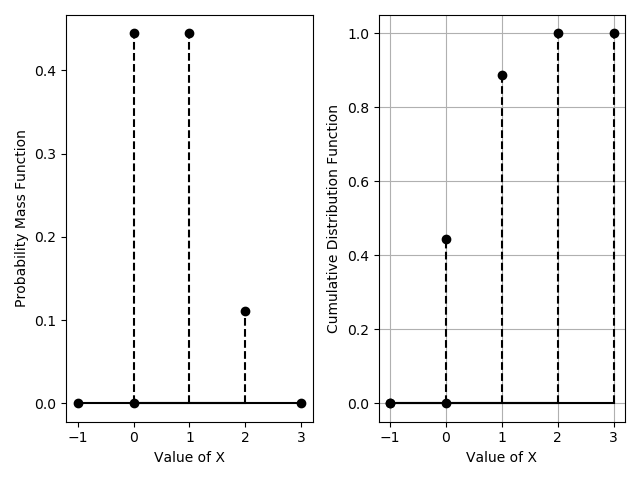
\includegraphics[width = 0.8\textwidth]{pfigs/f1.png}
	\end{center}
\end{frame}

\begin{frame}
\centering
\ \\ \ \\
\huge The End
\end{frame}

\end{document}